\documentclass{article} %选择文档类型,我们如果是做期末大作业的话选article就可以了

%正如c++需要import库来实现各种各样的功能,Latex也需要调用宏包来实现各种各样的功能
\usepackage{amsmath}  %调用公式宏包
\usepackage{graphicx} %调用插图宏包
\usepackage{ctex}     %调用中文宏包
\usepackage{listings}
\usepackage{fancyhdr} %调用页眉页脚宏包
\usepackage{listings}
\usepackage{xcolor}
\usepackage[table]{xcolor}
\usepackage{amsmath}
\usepackage{subfigure}
\usepackage{graphicx}
\usepackage{booktabs}
\usepackage{float}
\usepackage{hyperref}
\usepackage{placeins} %避免图片乱跑,要在图片后面加上\FloatBarrier
\pagestyle{fancy} %设置页面风格为fancy
\setCJKmainfont{FandolSong}
% \lstset{
%   language=R,
%   frame=single,
%   framesep=5pt,
%   framerule=0.5pt,
%   backgroundcolor=\color{white},
%   basicstyle=\ttfamily\small,
%   keywordstyle=\color{blue},
%   stringstyle=\color{purple},
%   commentstyle=\color{green!70!black},
%   rulecolor=\color{black},
%   breaklines=true,
%   postbreak=\mbox{\textcolor{red}{$\hookrightarrow$}\space},
%   showstringspaces=false
% }

\lstset{
  language=R, % 设置语言
  basicstyle=\small\ttfamily, % 设置字体族
  breaklines=true, % 自动换行
  keywordstyle=\bfseries\color{blue}, % 设置关键字为粗体,颜色为 NavyBlue
  morekeywords={}, % 设置更多的关键字,用逗号分隔
  emph={self}, % 指定强调词
  emphstyle=\bfseries\color{Rhodamine}, % 强调词样式设置
  commentstyle=\itshape\color{black!50!white}, % 设置注释样式,斜体,浅灰色
  stringstyle=\bfseries\color{blue}, % 设置字符串样式
  breaklines=true,
  columns=fullflexible,
%   numbers=left, % 显示行号在左边
%   numbersep=2em, % 设置行号的具体位置
  numberstyle=\footnotesize, % 缩小行号
%   frame=single, % 边框
  framesep=1em, % 设置代码与边框的距离
  backgroundcolor=\color{gray!5} % 设置背景颜色为浅灰色
}
%清除默认的页眉和页脚
\fancyhf{} 

\newcommand{\subsubsubsection}[1]{\paragraph{#1}\mbox{}\\}
\setcounter{secnumdepth}{4} % how many sectioning levels to assign numbers to
\setcounter{tocdepth}{4} % how many sectioning levels to show in ToC

%设置页眉内容
\lhead{Phlinsia} %左侧页眉内容
\rhead{时间序列分析课程总结} %右侧页眉内容

\fancyfoot[C]{第 \thepage 页} % 右侧页脚设置为页码
%\begin{document}这句话之前是导言区,这句话以后就开始写正文了
%可以把导言区理解为int main()函数之前的内容,而正文就是int main()主函数的部分了
\begin{document}




%标题封面部分
\begin{titlepage}
    \begin{center}
        \begin{figure}[H]
            \centering
            
\includegraphics[width=0.7\textwidth]{./pic/校名.pdf}
          \end{figure} 
          \huge \textbf{时间序列分析课程总结} \\ 
          \large \textbf{2023/2024(2)}
          \vspace{1cm}
          \begin{figure}[H]
            \centering
            
\includegraphics[width=0.3\textwidth]{./pic/校徽.pdf}
          \end{figure}

          \vspace{2.3cm}

          \large 学生班级\hspace{0.5cm}\underline{\makebox[5.5cm]{大数据分析2101班}} \\
          \vspace{0.2cm}
            \large 学生姓名\hspace{0.5cm}\underline{\makebox[5.5cm]{Phlinsia}} \\
            \vspace{0.2cm}
            \large 学生学号\hspace{0.5cm}\underline{\makebox[5.5cm]{202103150503}} \\ 
            \vspace{0.2cm}
            \large 成\quad 绩 \hspace{0.8cm}\underline{\makebox[5.5cm]{}} \\ 
            \vspace{2.5cm}
            \Large \heiti{理学院}
        \end{center}
\end{titlepage}

\clearpage % 避免标题页和正文之间的重叠


\tableofcontents
\listoffigures
\listoftables
\newpage


\section{时间序列的预处理}
\subsection{概率分布}
任意给定的有限维分布决定了整个时间序列的统计特性。

\textbf{概率分布的局限性}
\begin{enumerate}
    \item 仅有样本数据,不了解整体特性。
    \item 有限维分布通常只能近似,且特殊分布才能写出来。高维则很难写出分布函数。
    \item 计算复杂,不易估计。
\end{enumerate}

\subsection{特征统计量的基本概念}
\begin{itemize}
\item 均值函数
  \(\mu_t=E(X_t)\),一般地,不同时刻 \(\mu_t\) 可能取不同的值
\item 方差函数
  \(\sigma_t^2=Var(X_t)\)
\item 自协方差函数(\texttt{Cov})
  \[
  \gamma_{t,s}=Cov(X_t,X_s)=E(X_t,X_s)-\mu_t\mu_s
  \]
  t和s均为时刻。同一时间序列不同时间点,度量过去对现在的影响。
\item 自相关函数(\texttt{ACF})
  \[
  \rho_{t,s}=Corr(X_{t},X_{s})=\frac{\gamma_{t,s}}{\sqrt{\gamma_{t,t}\gamma_{s,s}}}
  \]
  t和s均为时刻。可利用样本估计总体,且估计较为精确。
  
\item \textbf{结论:}
  \[
  \mathrm{Cov}\left[\sum_{i=1}^{m}c_{i}Y_{t_{i}} ,\sum_{j=1}^{n}d_{j}Y_{s_{j}}\right]=\sum_{i=1}^{m}\sum_{j=1}^{n}c_{i}d_{j}\mathrm{Cov}(Y_{t_{i}},Y_{s_{j}})
  \]
  \[
  \mathrm{Var}\left[ \sum_{i=1}^{n}c_{i}Y_{t_{i}}\right]= \sum_{i=1}^{n}c_{i}^{2} \mathrm{Var}(Y_{t_{i}})+2\sum_{i=2}^{n}\sum_{j=1}^{i-1}c_{i}\mathrm{c}_{j}\mathrm{Cov}(Y_{t_{i}},Y_{t_{j}})
  \]
\end{itemize}

\subsection{平稳时间序列}
指的是统计特性随时间平移不变,泛指严平稳和宽平稳,偶尔也特指宽平稳。

\textbf{严平稳}

又称强平稳性。任意有限维分布斗鱼初始时间点无关,只与时间间隔相关。
分布函数随时间平移不变,即所有的统计性质均不会随时间变化

\textbf{严平稳性质}
\[
\begin{cases}
\gamma_0=Var(Y_t), & \rho_0=1 \\
\gamma_k=\gamma_{-k}, & \rho_k=\rho_{-k} \\
|\gamma_k|\leq\gamma_0, & |\rho_k|\leq 1
\end{cases}
\]

\textbf{宽平稳及其条件}

\begin{enumerate}
  \item 均值为常数,不随着t的变化而变化。
\item 一二阶矩存在。保证方差有限,即方差存在。  
\item 自协方差仅仅依赖于时间间隔,为T的函数。 
\end{enumerate}



\subsubsection{平稳时间序列的统计量性质}

\begin{itemize}
    \item 均值函数和方差函数都是常数。    \(\mu_t=\mu,\quad \sigma_t^2=\sigma^2\)
    \item 自相关和自协方差函数只依赖于时间间隔T,与时间起止点无关
          \item 延迟k自协方差函数
            \[
              \text{Cov}(X_t,X_{t+k})=\gamma(k)=\gamma_k=\gamma(t,t+k)
            \]
          \item 延迟k自相关函数
            \[
            \rho_k=\frac{\gamma(t,t+k)}{\sqrt{D(X_t)D(X_{t+k})}}=\frac{\gamma_k}{\gamma_0}=\frac{Cov(X_t,X_{t-k})}{Cov(X_t,X_t)}=\frac{E(X_t-\mu)(X_{t-k}-\mu)}{E(X_t-\mu)(X_t-\mu)}
            \]
      \end{itemize}

      \subsubsection{平稳性检验方法}

      \textbf{时序图直观检验}

      时序图提供了一个直观的方法来初步判断时间序列的平稳性。
      \begin{itemize}
          \item \textbf{均值稳定:} 若序列值在某常数值附近波动,表明序列的均值\(\mu\)可能是稳定的。
          \item \textbf{方差恒定:} 当序列的波动范围有界,且无显著的趋势或周期性特征时,暗示序列的方差\(\sigma^2\)可能保持恒定。
      \end{itemize}
      
      \textbf{自相关图分析}

      自相关图强调序列值之间的线性依赖关系仅取决于时间间隔:
      \begin{itemize}
          \item 在足够大的时间间隔\(\texttt{k}\)下,如果自相关系数逐渐衰减至零,这表明序列展现出强烈的短期相关性,而长期依赖性较弱。
          \item 自相关系数应遵循正态分布。
      \end{itemize}
      
      \textbf{单位根检验}

      为了更精确地判断时间序列的平稳性,单位根检验提供了一系列定量工具,通过数学模型检测序列是否存在单位根,从而判断序列是否非平稳。常见的单位根检验方法包括:
      \begin{itemize}
          \item \textbf{Dickey-Fuller (DF)检验:} 最早提出的一种单位根检验方法,适用于无趋势和无截距项的简单模型。
          \item \textbf{Augmented Dickey-Fuller (ADF)检验:} DF检验的扩展,引入了滞后项以更好地拟合序列的动态特性。
          \item \textbf{Phillips-Perron (PP)检验:} 另一种流行的单位根检验方法,它考虑了序列的异方差性和长记忆效应。
      \end{itemize}
      

\subsubsection{纯随机性检验(白噪声序列)}
平稳且非纯随机的时间序列才有研究价值。

\textbf{白噪声序列的定义和性质}
\begin{itemize}
\item \(\forall t\in T,E(X_t)=\mu\quad\)
\item \(\forall t,s\in T,r(t,s)=\begin{cases}t^2&t=s\\0&t\neq s\end{cases}\quad\text{即}\gamma_k=\begin{cases}\sigma_e^2 & k=0\\ 0 & k>0 \end{cases} \)
\item 自相关函数:\(\rho(t,s)=\begin{cases}1&t=s\\0&t\neq s\end{cases}\quad\text{即} \rho_k=\begin{cases}1 & k=0\\ 0 & k>0 \end{cases}\)
\end{itemize}

二阶矩$E(X^2)$存在(均值、方差都有时,二阶矩存在),是弱平稳序列。

\subsubsection{随机游动序列}

非平稳,形如\(Y_t=e_1+e_2+\cdots+e_t\)
其统计量为
\[\begin{gathered}
  \mu_t=t\cdot \mu,\quad \sigma_t^2=t\cdot \sigma_e^2\\
  \gamma_{t,s}=\min(t,s)\cdot \sigma_e^2\\
   \rho_{t,s}=\frac{\sqrt{\min(t,s)}}{\sqrt{\max(t,s)}}
\end{gathered}\]


\section{平稳时间序列分析}

\subsection{方法工具}

\subsubsection{差分运算}

\textbf{一步差分}
\begin{enumerate}
\item 一阶差分
  \[
  \nabla X_t=X_{t}-X_{t-1}
  \]
\item 二阶差分
  \[
  \nabla^{2}X_{t}=\nabla X_{t}-\nabla X_{t-1}=(X_{t}-X_{t-1})-(X_{t-1}-X_{t-2})=X_{t}-2X_{t-1}+X_{t-2}
  \]
\item \texttt{p}阶差分
  \[
  \nabla^pX_t=\nabla^{p-1}X_t-\nabla^{p-1}X_{t-1}
  \]
\end{enumerate}

\textbf{\texttt{k}步差分}
\[
\nabla_kX_t=X_t-X_{t-k}
\]

\subsubsection{延迟算子\texttt{B}}

\begin{enumerate}
\item 类似于一个时间指针,当序列值乘\texttt{k}个延迟算子,即把序列值时间向过去拨了\texttt{k}个时刻。
  \[
  \begin{aligned}
  &X_{t-1}=BX_{t}\\
  &X_{t-2}=B^{2}X_{t}\\
  &\quad\quad\cdots\\
  &X_{t-p}=B^{p}X_{t}
  \end{aligned}
  \]
\item 用\texttt{B}表示差分
  \begin{itemize}
  \item \texttt{p}阶差分:
    \[
    \nabla^pX_t=(1-B)^pX_t=\sum_{i=0}^p(-1)^pC_p^iX_{t-i}
    \]
    \[
    \begin{aligned}
    &\nabla X_{t}=X_{t}-X_{t-1}=(1-B)X_{t}\\
    &\nabla^{2}X_{t}=\nabla X_{t}-\nabla X_{t-1}=(1-B)X_{t}-(1-B)X_{t-1}=(1-B)^{2}X_{t}\\
    &\quad\quad\quad\quad\quad\quad\quad\quad\quad\quad\quad\quad\quad\quad\cdots\\
    &\nabla^{P}X_{t}=(1-B)^{P}X_{t}
    \end{aligned}
    \]
  \item \texttt{k}步差分:
    \[
    \nabla_kX_t=(1-B^k)X_t=X_t-X_{t-k}
    \]
  \end{itemize}
\end{enumerate}

\subsection{\textbf{AR}和\textbf{MA}模型}

\textbf{ARMA}模型为自回归滑动平均混合模型。

\subsubsection{\textbf{Wold}分解定理}
\textbf{奠定了\textbf{ARMA}模型的理论基础},即对任意的离散平稳序列$\{X_t\}$,可分解为2个不相关的平稳序列之和。这一分解揭示了序列的确定性成分与随机成分之间的基本联系。

\[X_t=\phi_1X_{t-1}+\phi_2X_{t-2}+\cdots-\varepsilon_t\]

前面与$X_t$有关的是确定性序列,后面$\varepsilon_t$是随机序列。

\subsubsection{一般线性过程}

可以表示为现在和过去白噪声变量的加权线性组合。

\[Y_t=e_t+\psi_1 e_{t-1} +\psi_2 e_{t-2} + \cdots\]

\subsubsection{AR模型(自回归过程)}
\textbf{AR(p)}:称为p阶自回归模型

\textbf{AR(1)}
\[
X_t=\phi_1 X_{t-1}+\varepsilon_t
\]

\begin{itemize}
\item $X_t$:中心化后的平稳序列($\mu=0$)
\item $\phi_1$:$X_{t-1}$对$X_t$的影响
\item $\varepsilon_t$:随机扰动
\end{itemize}

如果AR(1)模型的特征根\(|\phi_1|<1\),则序列平稳。
\[
  \begin{gathered}
\mu=\frac{0}{1-\phi}=0,\quad \gamma_0=\frac{\sigma^2_e}{1-\phi^2}\geq 0,\quad Cov(\varepsilon_t,X_s)=0 \\
  Cov(X_t,X_{t-k})=\phi^k \gamma_0 ,\quad \rho_k=\phi^k \quad \text{(指数衰减)}
\end{gathered}
\]

\textbf{AR(2)二阶自回归模型}
\[
  \begin{gathered}
  X_t=\phi_1 X_{t-1}+\phi_2 X_{t-2}+e_t\\
  \mu=\frac{0}{1-\phi_1-\phi_2}=0,\quad \gamma_0=\frac{\sigma^2_e 1-\phi_2}{(1+\phi_2)[(1+\phi_2)^2-\phi_1^2]} \\
  \rho_1=\frac{\phi_1}{1-\phi_2},\quad \gamma_1=\rho_1\gamma_0\\
  \end{gathered}
\]

\textbf{Yule-Walker方程}

描述了\textbf{AR}模型的自协方差函数如何递归地依赖于模型参数。

\[
  \begin{gathered}
    Cov(X_t,X_{t-k})=Cov(\phi_1 X_{t-1}+\phi_2 X_{t-2}+\varepsilon_t,X_{t-k})\\
    \begin{cases} \gamma_k=\phi_1\gamma_{k-1}+\phi_2\gamma_{k-2},\quad k\geq 2\\
      \rho_k=\phi_1\rho_{k-1}+\phi_2\rho_{k-2},\quad k\geq 2
    \end{cases}
    \end{gathered}
\]
\begin{itemize}
  \item 对于\(\rho_k\)随着k增加而指数衰减。
  \item ACF有不同模式,取决于根是复数还是实数。
\end{itemize}

\subsubsection{AR(p)}

\textbf{定义}
\[
X_t=\phi_0+\phi_1X_{t-1}+\phi_2X_{t-2}+\cdots+\phi_pX_{t-p}+\varepsilon_t, \quad \phi_p\not=0
\]

\textbf{性质}
\begin{itemize}
\item $E(\varepsilon_t)=0$
\item $Var(\varepsilon_t)=\sigma_{\varepsilon}^2$
\item $Cov(\varepsilon_t,\varepsilon_s)=0\quad s\not =t$, 随机扰动项是均值为0的白噪声
\item $Cov(X_s,\varepsilon_t)=0$
\item 当$\phi_0=0$时(常数项为0),为中心化的AR(p)模型
\end{itemize}

\textbf{中心化变换(去掉常数项)}

若$\phi_0\not =0$,令$\mu=\dfrac{\phi_0}{1-\phi_1-\phi_2-\cdots-\phi_p}$

去中心化后:
\[
Y_t=X_t-\mu
\]

\textbf{自回归系数多项式}
\[
X_t=\phi_0+\phi_1X_{t-1}+\phi_2X_{t-2}+\cdots+\phi_pX_{t-p}+\varepsilon_t
\]
\[
\Rightarrow \quad \varepsilon_t=(1-\phi_1B-\phi_2B^2-\cdots-\phi_pB^p)X_t=\phi(B)X_t
\]
\[
\Rightarrow \quad \phi(B)X_t=\varepsilon_t
\]

\textbf{AR(p)平稳性判别}

图示判别直观,但准确度不高。特征根判别更准确。

\textbf{特征根判别}

\begin{enumerate}
\item 写出特征根
\[
X_t-\phi_1X_{t-1}-\phi_2X_{t-2}-\cdots-\phi_pX_{t-p}=\varepsilon_t
\]
\[
\Rightarrow \lambda^p-\phi_1\lambda^{p-1}-\phi_2\lambda^{p-2}-\cdots-\phi_p\lambda^0=0
\]
\item 判断
\begin{itemize}
\item $\lambda(p)$的$p$个特征根都在单位圆内,$|\lambda|<1$
\item $\phi(\mu)=0$(自回归多项式)的根都在单位圆外,$\lambda=\frac{1}{B}\quad |B|>1$
\end{itemize}
\end{enumerate}

\textbf{平稳域判别}

$\phi_1,\phi_2,\cdots,\phi_p$特征根在圆内,主要考察一阶、二阶
\begin{itemize}
\item AR(1)
\[
\lambda=\phi_1,|\phi_1|<1,
\]
即$\{\phi_1|-1<\phi_1<1\}$
\item AR(2)
\[
X_t=\phi_1X_{t-1}+\phi_2X_{t-2}+\varepsilon_t\Rightarrow\lambda^2-\phi_1\lambda_1-\phi_2=0
\]
\[
\lambda=\dfrac{\phi_{1}\pm\sqrt{\phi_{1}^{2}+4\phi_{2}}}{2},\quad |\lambda_{1}|<1,|\lambda_{2}|<1
\]
即平稳域为$\{\phi_1,\phi_2||\phi_2|<1且\phi_2\pm\phi_1<1\}$
\end{itemize}

\textbf{平稳AR模型的统计性质}
\begin{enumerate}
\item 均值
\begin{itemize}
\item 非中心化:$\mu=\dfrac{\phi_0}{1-\phi_1-\phi_2-\cdots-\phi_p}$
\item 中心化:$\mu = 0$
\end{itemize}
\item 方差
\begin{itemize}
\item 整个的AR模型的方差
\(
AR(1):\dfrac{\sigma_e^2}{1-\phi_1^2}
\)
\item 用作预测
\[
\begin{aligned}
G_0&=1\\
G_1&=\phi_1\\
G_2&=\phi_1^2\\
G_3&=\phi_1^3\\
G_4&=\phi_1^4\\
\cdots
\end{aligned}
\]
\[
\begin{aligned}
G_0&=1\\
G_1&=\phi_1G_0\\
G_2&=\phi_1G_1+\phi_2G_0\\
G_3&=\phi_1G_2+\phi_2G_1\\
G_4&=\phi_1G_3+\phi_2G_2\\
\cdots
\end{aligned}
\]
\[
\Rightarrow Var(X_t)=(G_0^2+G_1^2+G_2^2+\cdots)\sigma_e^2
\]
\[
\begin{aligned}
Var(X_{t-0})&=G_0^2\sigma_e^2\\
Var(X_{t-1})&=(G_0^2+G_1^2)\sigma_e^2\\
Var(X_{t-2})&=(G_0^2+G_1^2+G_2^2)\sigma_e^2\\
\cdots
\end{aligned}
\]
\end{itemize}
\item 协方差函数
\begin{itemize}
\item $AR(1):r_k=\phi_1^k\dfrac{\sigma_e^2}{1-\phi_1^2}$
\item $AR(2):\begin{cases}
r_{0}=\dfrac{1-\phi_{2}}{(1+\phi_{2})(1-\phi_{1}-\phi_{2})(1+\phi_{1}-\phi_{2})}\sigma_e^2\\
r_{1}=\dfrac{\phi_{1}r_{0}}{1-\phi_{2}}\\
r_{k}=\phi_{1}r_{k-1}+\phi_{2}r_{k-2},\quad k\geq2
\end{cases}$
\end{itemize}
\item 自相关系数
\begin{itemize}
\item 拖尾性、呈指数衰减
\[
\rho_k=\dfrac{r_k}{r_0}
\]
\[
\rho_{k}=\phi_{1}\rho_{k-1}+\phi_{2}\rho_{k-2}+\cdots+\phi_{p}\rho_{k-p}
\]
\[
AR(1):\quad \rho_{k}=\dfrac{r_{k}}{r_{0}}=\phi_{1}^{k}
\]
\[
AR(2):\quad\rho_{k}=\frac{r_{k}}{r_{0}}=\begin{cases}
1&k=0\\
\dfrac{\phi_{1}}{1-\phi_{2}}&k=1\\
{\phi_{1}\rho_{k-1}+\phi_{2}\rho_{k-2}}&k\geq2
\end{cases}
\]
\end{itemize}
\item 偏自相关系数
\begin{itemize}
\item 剔除了中间 $k-1$ 个随机变量的干扰,$X_{t-k}$ 对 $X_t$ 影响的相关度量(单纯度量两变量间的相关性,而自相关则有两时刻中间的相关度量)
\[
AR(1):\quad\phi_{kk}=\begin{cases}
\phi_{1}&k=1\\
0&k\geq 2
\end{cases}
\]
\[
AR(2):\quad \phi_{kk}=\begin{cases}
\dfrac{\phi_{1}}{1-\phi_{2}}&k=1\\
\phi_{2}&k=2\\
0&k\geq3
\end{cases}
\]
\[
p\,阶截尾:\phi_{kk}=0,\quad k>p
\]
对$AR(1):\phi_{11}\not =0$,其他均为0
对 $AR(2):\phi_{11},\phi_{22}\not = 0$,其他均为0
\end{itemize}
\end{enumerate}



\subsubsection{MA模型(滑动平均过程)}

\textbf{定义}
\[
\begin{cases}
X_t=\varepsilon_t-\theta_1\varepsilon_{t-1}-\theta_2\varepsilon_{t-2}-\cdots-\theta_q\varepsilon_{t-q}\\
\theta_q\not=0
\end{cases}
\]
\[
\begin{aligned}
X_t&=\varepsilon_t-\theta_1\varepsilon_{t-1}-\cdots-\theta_q\varepsilon_{t-q}\\
&=\varepsilon_t-\theta_1B\varepsilon_t-\cdots-\theta_qB^q\varepsilon_t\\
&=ⒽB\varepsilon_t
\end{aligned}
\]
\[
 \text{Hanson} B=1-\theta_1B-\theta_2B^2-\cdots-\theta_qB^q \quad (\text{移动平均系数多项式})
\]

\textbf{统计性质}
\begin{enumerate}
\item {常数均值}
\(
E(X_t)=\mu
\)

\item {常数方差}
\(
var(X_t)=(1+\theta_1^2+\cdots+\theta_q^2)\varepsilon_q^2
\)

\item \textbf{自协方差$q$阶截尾}
\[
r_{k}=\begin{cases}
(1+\theta_{1}^{2}+\cdots+\theta_{q}^{2})\sigma_e^{2},&k=0\\
(-\theta_{k}+\sum_{i=1}^{q-k}\theta_{i}\theta_{k+i})\sigma_e^{2},&1\leq k\leq q\\
0,&k>q
\end{cases}
\]

\[
\text{MA}(1):\begin{cases}
(1+\theta_1^2)\sigma_e^2&k=0\\
-\theta_1\sigma_e^2&k=1\\
0&k>1
\end{cases}
\]
\[
\begin{aligned}
  \text{MA}(2):\begin{cases}
(1+\theta_{1}^{2}+\theta_2^2)\sigma_e^{2}&k=0\\
(-\theta_{1}+\theta_{1}\theta_{2})\sigma_e^{2}&k=1\\
-\theta_{2}\sigma_e^{2}&k=2\\
0&k\geq3
\end{cases}
\end{aligned}
\]

\item \textbf{自相关系数$p$阶截尾}
\[
  \text{MA}(1):\quad\rho_k=\left\{\begin{array}{ll}
1,&\text{if }k=0\\
-\dfrac{\theta}{1+\theta^2},&\text{if }k=1\\
0,&\text{if }k\ge2
\end{array}\right.
\]
\[
  \text{MA}(2):\quad \left.\rho_k=\left\{\begin{array}{ll}
1,&\quad\text{if }k=0\\
\dfrac{-\theta_1+\theta_1\theta_2}{1+\theta_1^2+\theta_2^2},&\quad\text{if }k=1\\
\dfrac{-\theta_2}{1+\theta_1^2+\theta_2^2},&\quad\text{if }k=2\\
0,&\quad\text{if }k\geq3
\end{array}\right.\right.
\]

\end{enumerate}

\subsubsection{MA的可逆性}

有限阶$\text{MA}$模型一定平稳。

\textbf{$\text{MA}(q)$的可逆条件}
\[
  \text{MA}(1):\quad |\theta_1|<1
\]
\[
  \text{MA}(2):\quad |\theta_2|<1\quad\theta_2\pm\theta_1<1
\]

\textbf{MA模型的判别}
\begin{itemize}
\item 自相关系数$q$阶截尾$\Rightarrow MA(q)$
\item 偏自相关系数$\infty$阶截尾 (拖尾)
\end{itemize}

\subsection{\textbf{ARMA}模型(自回归移动平均)}

\subsubsection{\textbf{ARMA}(p,q)}
\[
\begin{cases}
x_{t}=\phi_{0}+\phi_{1}x_{t-1}+\cdots+\phi_{p}x_{t-p}+\varepsilon_{t}-\theta_{1}\varepsilon_{t-1}-\cdots-\theta_{q}\varepsilon_{t-q}\\
\phi_{p}\not =0\quad\theta_{q}\neq0\\
E(\varepsilon_{t})=0,Var(\varepsilon_{t})=\sigma_{\varepsilon}^{2},E(\varepsilon_t \varepsilon_{s})=0\quad s\neq t\\
E(x_{t}\varepsilon_{t})=0,s<t
\end{cases}
\]
$\phi_0=0$时,中心化的\textbf{ARMA}(p,q)模型

\subsubsection{系数多项式}
用滞后算子$B$表示,其中\(\Phi(B)\) 和 \(\Theta(B)\) 分别是 AR 和 MA 部分的多项式。AR部分决定平稳,MA部分决定可逆。
\[
\begin{aligned}
\Phi(B)Y_{t}& =\Theta(B)e_t  \\
\Phi(B)& =1-\phi_1B-\phi_2B^2+\cdots-\phi_pB^p,  \\
\Theta(B)& =1-\theta_1B-\theta_2B^2+\cdots-\theta_qB^q
\end{aligned}
\]

\subsubsection{统计性质}

\textbf{均值}
\[
\mu=\dfrac{\phi_0}{1-\phi_1-\phi_2-\cdots-\phi_p}
\]

\textbf{协方差}
\[
r_k=\sigma_e^2\sum_{i=0}^{\infty}G_iG_{i+k}
\]

\textbf{自相关系数}
\[
\rho_k=\dfrac{\sum_{i=0}^{\infty}G_iG_{i+k}}{\sum_{i=0}^{\infty}G_i^2}
\]

\textbf{相关性}

\begin{table}[h]
\centering
\begin{tabular}{c|cc}
\hline
    模型     & 自相关系数 & 偏自相关系数 \\
\hline
   \texttt{AR(p)}   &    拖尾    &  \texttt{p}阶截尾   \\
   \texttt{MA(q)}   & \texttt{q}阶截尾  &     拖尾     \\
 \texttt{ARMA(p,q)} &    拖尾    &     拖尾     \\
\hline
\end{tabular}
\caption{不同模型的自相关和偏自相关特性}
\end{table}

\section{非平稳时间序列的分析}

\subsection{差分平稳}

\begin{table}[H]
  \centering
  
  \label{tab:differencing_choices}
  \begin{tabular}{|c|c|}
  \hline
  \textbf{趋势类型} & \textbf{差分策略} \\ \hline
  线性趋势       & 一阶差分         \\ \hline
  曲线趋势       & 低阶差分         \\ \hline
  固定周期趋势   & 步长为周期长度的差分运算 \\ \hline
  \end{tabular}
  \caption{差分方式的选择}
\end{table}

过差分可能导致有用的信息浪费,降低估计精度;且使方差增加。

\begin{table}[H]
  \centering
  \
  \begin{tabular}{|c|c|}
  \hline
  \textbf{方法} & \textbf{描述} \\ \hline
  对数变换     & 通过取对数压缩数据范围,减少异方差性。 \\ \hline
  幂变换       & 通过幂次变换调整数据分布,适用于多种非线性关系。 \\ \hline
  \end{tabular}
  \caption{非差分的平稳化方法}
\end{table}

\subsection{\texttt{ARIMA}模型(自回归差分滑动平均)}
\textbf{ARIMA(p,d,q)}
\[
W_t=\phi_1W_{t-1}+\phi_2W_{t-2}+\cdots+\phi_pW_{t-p}+e_t-\theta_1e_{t-1}-\theta_2e_{t-2}-\cdots-\theta_qe_{t-q}
\]
其中,\(W_t\) 是经过 \(d\) 次差分后的序列值,\(\phi_i\) 和 \(\theta_j\) 分别是自回归和移动平均模型的参数,\(e_t\) 表示随机误差项。

\section{模型拟合}

\subsection{参数估计}
选择好模型之后,下一步就是估计模型中未知参数的值。对于一个非中心化\texttt{ARMA(p,q)}模型,该模型共含有\( p+q+2 \)个未知参数:\[\phi_1,...,\phi_\mathrm{p},\theta_1,...,\theta_\mathrm{q},\mu,\sigma_\epsilon^2\]

其中参数\(\mu\)是序列均值,通常采用矩估计方法,用样本均值估计总体均值即可得到它的估计值。对剩下的\( p + q + 1 \) 个未知参数的估计方法有三种:矩估计、极大似然估计和最小二乘估计。

\subsection{残差检验}

\subsubsection{残差的无关性检验}

利用\texttt{Ljung-Box}对一阶差分序列的残差进行白噪声检验。
检验统计量为\texttt{LB}检验统计量。
原假设和备择假设分别为:
\[
\begin{gathered}
H_0:\rho_1=\rho_2=\cdots=\rho_m=0, \\
H_1:\exists k\leq m \quad \text{ s.t. } \rho_k \neq 0,
\end{gathered}
\]

\begin{itemize}
  \item 若\(p<0.05\),拒绝原假设,残差序列中还残留相关信息,拟合模型不显著,原始序列存在相关性
  \item 若\(p>=0.05\),接收原假设,原始序列独立,纯随机;残差是白噪声。
\end{itemize}

\subsubsection{残差的正态性检验}
残差的\texttt{QQ}图展示了残差分布与理论正态分布之间的对比,如果点大致沿45°线分布,则模型的残差满足正态性假设。

\subsubsection{参数的显著性检验}
参数显著性检验旨在确认模型中的每个参数是否显著非零。通过计算系数估计值与其标准误(\texttt{s.e.})的比值,即\texttt{t}统计量,与\texttt{t}分布的5\%临界值(1.96)进行比较。若该比值的绝对值超过1.96,则拒绝零假设,相应的自变量对模型有实质影响。

\subsubsection{模型优化}
同一个序列可以构造多个有效拟合模型。可引入\texttt{AIC}和\texttt{BIC}信息准则选出最佳模型。

\subsubsection{模型预测}
在\texttt{R}语言环境下,利用\texttt{forecast}函数,基于线性最小方差预测原则,未来序列值\(x_{t+1}\)被建模为历史数据\(x_t, x_{t-1}, \ldots\)的线性组合,以实现最小方差预测。尤其\texttt{ARIMA}模型在短期样本外预测中表现优异,但预测期\(k\)宜控制在模型参数\(p+q\)之内。预测虽无法消除未来不确定性,却能为决策者提供基于当前趋势的未来场景预览,故对其作用应持理性态度,既不过分低估也不过度依赖。
\begin{figure}[H] % 开始一个浮动体环境,[h]指定为 here(这里)位置
	\centering % 图片居中
	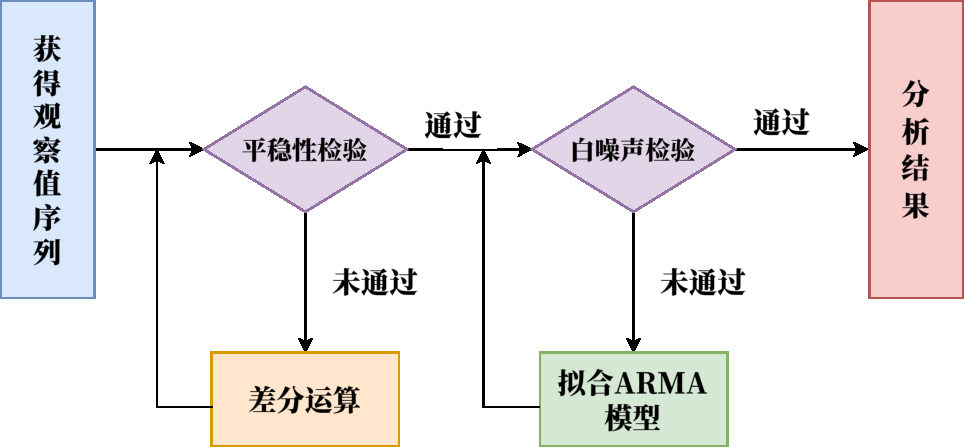
\includegraphics[width=\textwidth]{pic/ARIMA_new.pdf} % 插入宽度为文本宽度一半的图片
	\caption{ARIMA建模步骤} % 图片标题
	\label{} % 图片标签,用于引用
\end{figure}

% %分章节的示例,Latex会自动帮忙给标题编号
% \section{背景介绍}

% 在当今全球化金融市场背景下,股票价格波动性的研究已成为金融学领域的重要议题。随着市场复杂度与互联性的增强,股票价格的波动不仅受到宏观经济环境、企业财务表现、投资者情绪、政策调整及全球事件等多元因素的影响,更呈现出显著的非线性与随机性特征。这一复杂动态网络要求我们采用更加精细与系统的方法来解析其中的内在规律,以期提升投资决策的准确性与效率。

% 时间序列分析,作为一种强大的统计工具满足了这一需求。它通过对一系列按时间顺序排列的数据点进行分析,揭示出隐藏于数据背后的模式与趋势。在金融领域,尤其是针对股票价格的研究中,时间序列被定义为一连串在特定时间点上观测到的随机变量\(X(t)\)的样本实现\(\{X_{t_1}, X_{t_2},\cdots, X_{t_N}\}\),其中\(t_1, t_2, \cdots, t_N\)代表了离散的时间点。这种离散特性与股票市场的交易特性不谋而合,使得时间序列分析成为剖析股票价格波动的理想方法。

% 苹果公司,作为全球市值领先的科技巨头之一,其产品与服务覆盖了消费电子、软件开发、数字内容等多个关键领域,拥有庞大的用户基础与品牌忠诚度。因为苹果公司在全球科技产业中的独特地位与深远影响力,本文将聚焦于苹果公司股票价格的时间序列分析。


% \FloatBarrier

% \section{原始数据分析}

% \subsection{时序图}
% 在本节中,我们着手于对苹果公司股票价格数据进行直观的视觉呈现,旨在揭示其长期走势特征及潜在的时间序列属性。为此,我们精心构建了股票价格的时序图,这一图表生动地描绘了苹果公司股价自1990年2月1日至2011年10月14日间的演变轨迹(代码片段如列表所示)。

% \begin{lstlisting}
%     report <- read.csv("C:\\Users\\princ\\Desktop\\大三下\\时间序列分析\\课程设计\\report.csv")
%     report = ts(report)
%     Start <- as.Date('1990-2-1')
%     End <- as.Date('2011-10-14')
%     dt <- seq(from = Start, to = End, by = 1)
%     plot(report, main = 'Apple 股票趋势', xlab = '时间', ylab = '股价', type = 'o')
% \end{lstlisting}

% \begin{figure}[h] % 开始一个浮动体环境,[h]指定为 here(这里)位置
% 	\centering % 图片居中
% 	%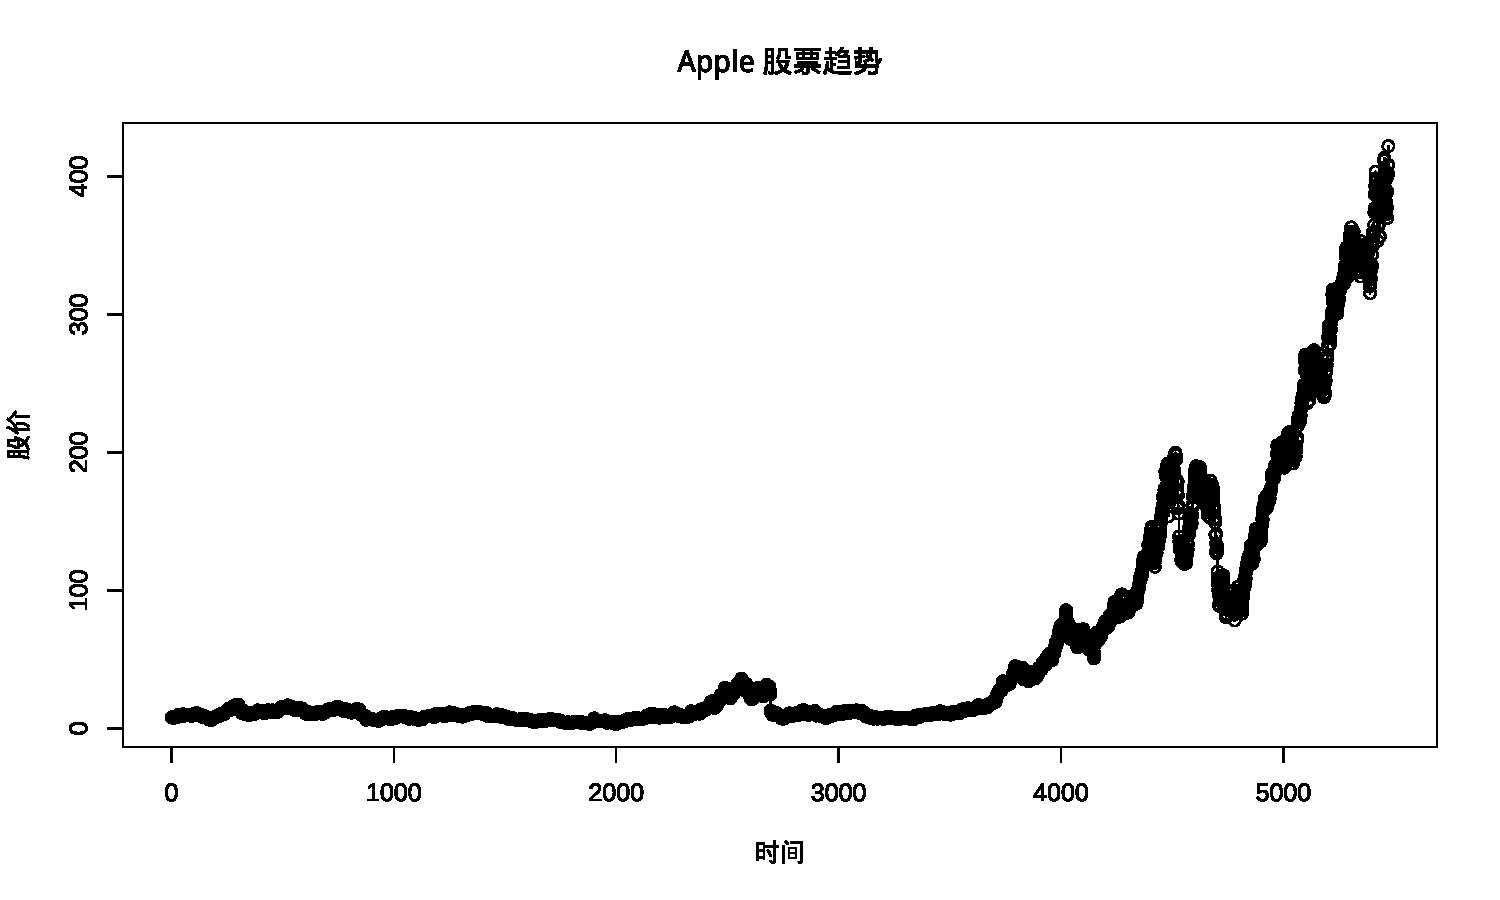
\includegraphics[width=\textwidth]{pic/Apple_stock_trend.pdf} % 插入宽度为文本宽度一半的图片
% 	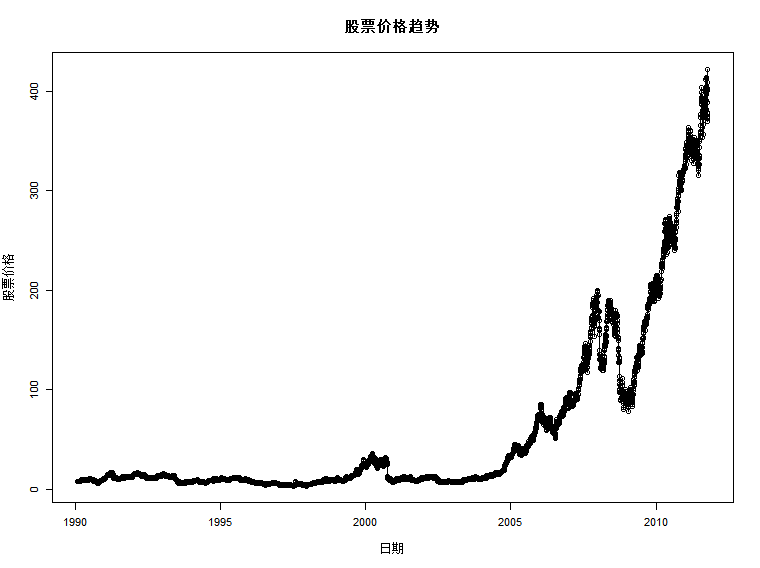
\includegraphics[width=\textwidth]{pic/stock.png}
%     \caption{苹果公司股票趋势时序图} % 图片标题
% 	\label{} % 图片标签,用于引用
% \end{figure}

% 早在1990年代初,苹果公司股票价格徘徊在一个相对较低的水平,大致位于100元左右。进入21世纪,苹果公司迎来了其发展历程中的转折点。随着技术创新与市场战略的成功实施,公司股票价格开始步入上升通道,至2000年前后,股价攀升至接近300元的高位。然而,在接下来的几年里,价格出现了大幅波动,有时甚至短暂回撤至200元左右。到了2005年左右,股票价格再次开始稳步上涨,并在2010年达到了一个新的高点,成功突破400元大关。然而,值得注意的是,在这期间穿插着多次短期回调与市场修正。

% 该时序图清晰地展现了苹果公司股票价格的长期上升趋势,这一发现暗示了序列的非平稳特性——即序列的均值随时间推移而发生显著变动,未能维持在某一恒定水平上。这一特性对于后续的时间序列分析至关重要,提示我们在进一步建模前需采取差分或其他平稳化手段以确保模型的有效性和预测精度。

% \FloatBarrier

% \subsection{Augmented Dickey-Fuller (ADF) 平稳性检验}

% 为进一步验证前述时序图中直观显示的非平稳特性,我们采用了Augmented Dickey-Fuller (ADF)检验,这是一种广泛应用的统计测试方法,用于评估时间序列的平稳性。ADF检验的核心在于检验序列是否存在单位根,从而判断其是否表现出随机游走特征。具体而言,ADF检验通过构建一个关于时间序列差分的回归模型来估计单位根的存在性,并基于回归结果计算出相应的统计量和p值,以此作为拒绝或接受原假设的依据。

% \begin{lstlisting}
%     adf.test(report)

%     ## Warning in adf.test(report): p-value greater than printed p-value
%     ##
%     ## Augmented Dickey-Fuller Test
%     ##
%     ## data: report
%     ## Dickey-Fuller = 1.5853, Lag order = 17, p-value = 0.99
%     ## alternative hypothesis: stationary
% \end{lstlisting}

% ADF检验的结果揭示了一个重要的事实:在本案例中,序列的p值高达0.99,远超过我们设定的显著性水平(通常为0.05)。这一结果明确指示我们无法拒绝原假设,即认为该时间序列是非平稳的,存在显著的单位根效应。换句话说,序列的均值并非固定不变,而是呈现出随时间变化的趋势,这与我们在时序图中观察到的长期上升趋势相吻合。


% \subsection{自相关图与偏自相关图分析}
% 在深入探讨时间序列的结构特征时,自相关图(Autocorrelation Function, ACF)与偏自相关图(Partial Autocorrelation Function, PACF)是不可或缺的分析工具。它们不仅能够揭示序列内部的依赖关系,还能为模型选择提供直观的指导。基于这一认识,我们对苹果公司股票价格序列进行了ACF与PACF的细致分析,以进一步探究其平稳性与潜在的自回归与移动平均特性。

% 接下来,我们根据自相关图和偏自相关图粗略判断序列是否平稳。若自相关图和偏自相关图里的系数很快地衰减为 0,则说明序列平稳,否则为非平稳。

% \begin{lstlisting}
%     # 自相关函数
%     acf(as.vector(report), lag.max = 500)

%     # 偏自相关函数
%     pacf(as.vector(report), lag.max = 300)
% \end{lstlisting}

% \begin{figure}[h] % 开始一个浮动体环境,[h]指定为 here(这里)位置
% 	\centering % 图片居中
% 	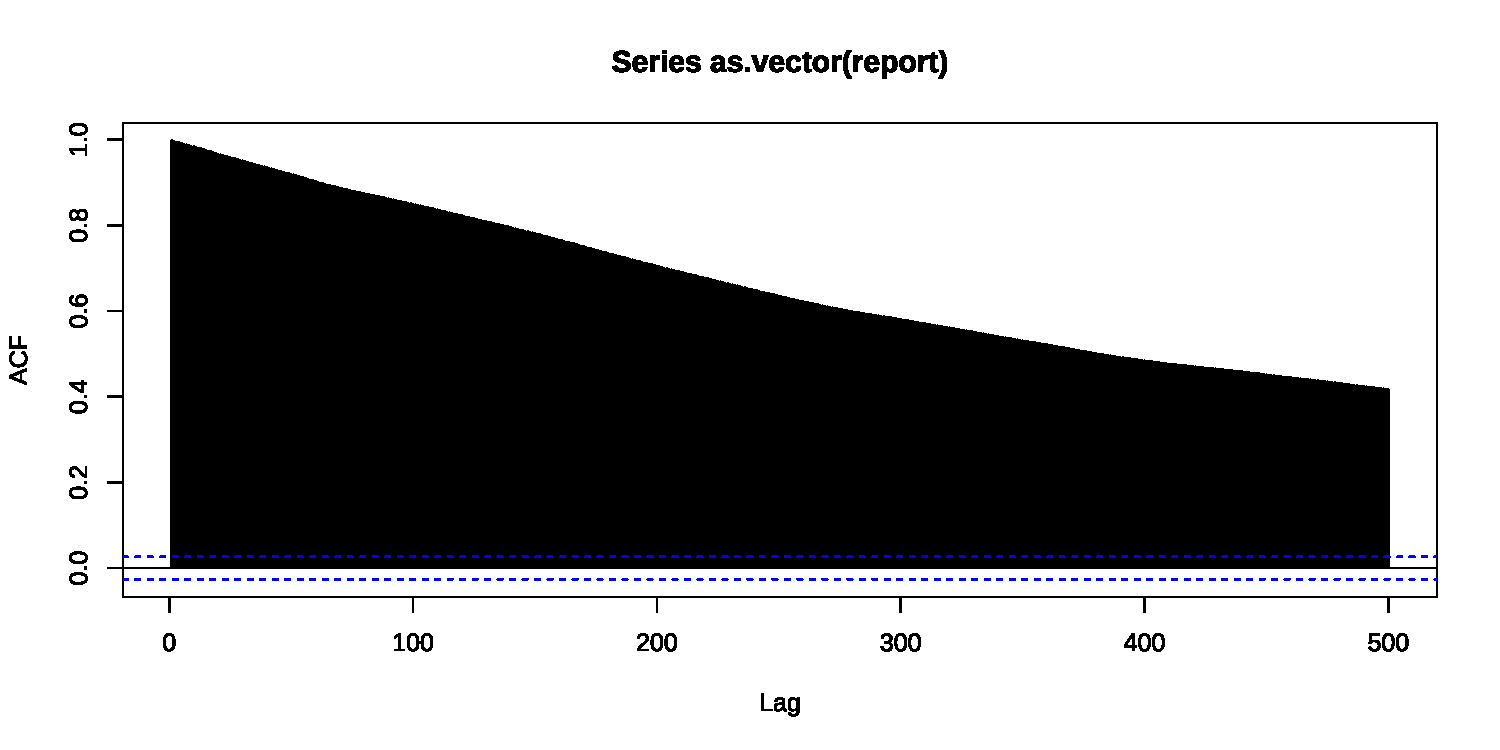
\includegraphics[width=\textwidth]{pic/acf.pdf}
%     \caption{原始数据自相关图} % 图片标题
% 	\label{} % 图片标签,用于引用
% \end{figure}

% \begin{figure}[h] % 开始一个浮动体环境,[h]指定为 here(这里)位置
% 	\centering % 图片居中
% 	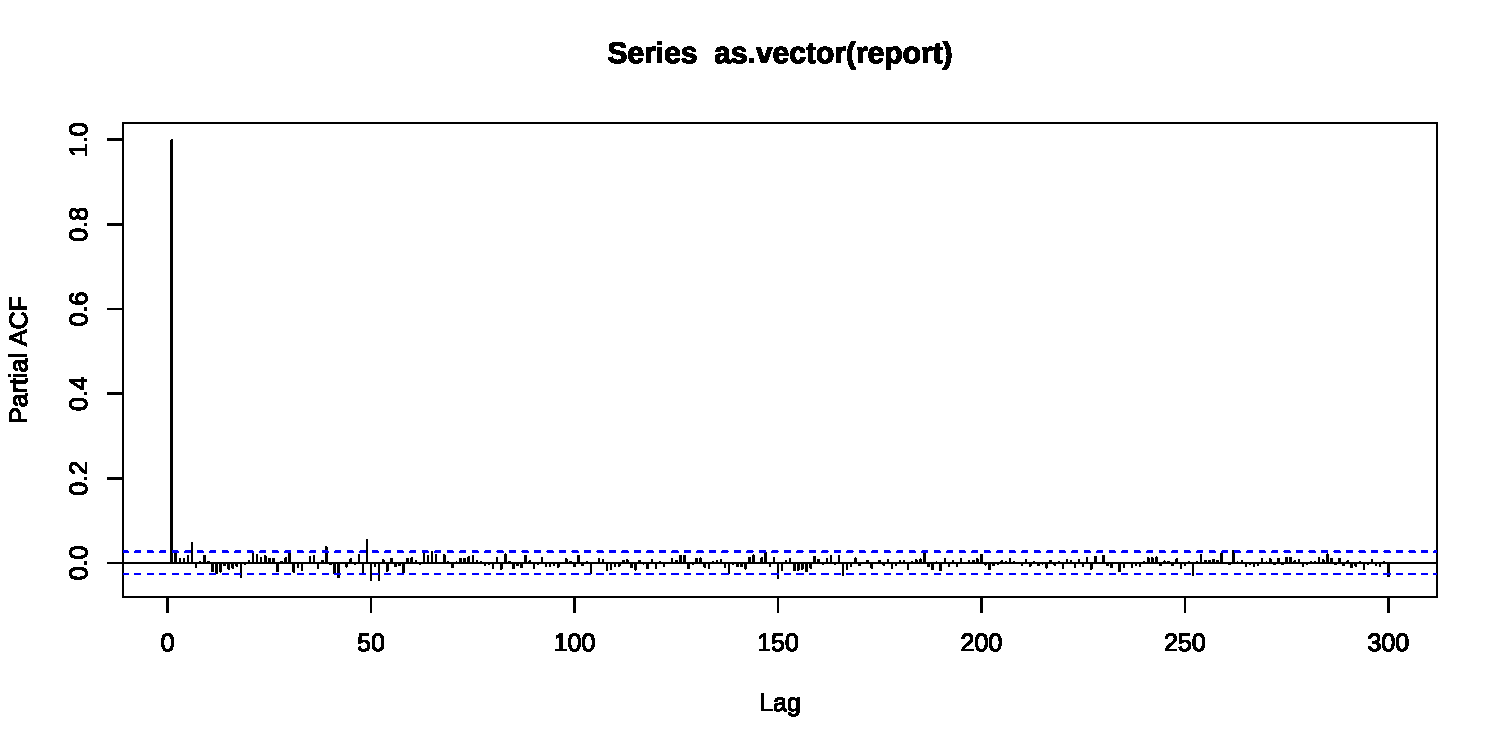
\includegraphics[width=\textwidth]{pic/pacf.pdf}
%     \caption{原始数据偏自相关图} % 图片标题
% 	\label{} % 图片标签,用于引用
% \end{figure}

% \FloatBarrier

% 通过仔细观察自相关图与偏自相关图,我们发现苹果公司股票价格序列展现出显著的非平稳性特征。具体而言,自相关图中的系数并未迅速衰减至零,反而呈现出较为持久的拖尾现象,这与理论上平稳序列的自相关系数在零附近徘徊的行为形成鲜明对比。同样,偏自相关图亦未显示出迅速收敛的迹象,进一步证实了序列的非平稳性质。此外,自相关图中部分系数超过了置信区间(通常以两倍标准误差表示,即图中蓝色虚线),这强烈暗示序列中存在显著的自相关性,而非随机白噪声。

% 综合以上分析,我们可以确信苹果公司股票价格序列在未经任何预处理的情况下是非平稳的。


% \section{平稳化处理}

% 若序列为非平稳,则需将序列通过差分转化为平稳序列。差分可以消除序列的线性趋势以及周期性。

% \subsection{一阶差分消除趋势}

% \begin{lstlisting}
%     # 一阶差分,消除整体上升趋势
%     plot(diff(report, 1), ylab = '1st Diff. of report', xlab = 'day', type = 'o')
% \end{lstlisting}

% 画出一阶差分序列的时序图,观察序列是否平稳。利用 acf()函数。画出一阶差分序列的自相关图,通过自相关图判断序列是否平稳。

% \begin{figure}[h] % 开始一个浮动体环境,[h]指定为 here(这里)位置
% 	\centering % 图片居中
% 	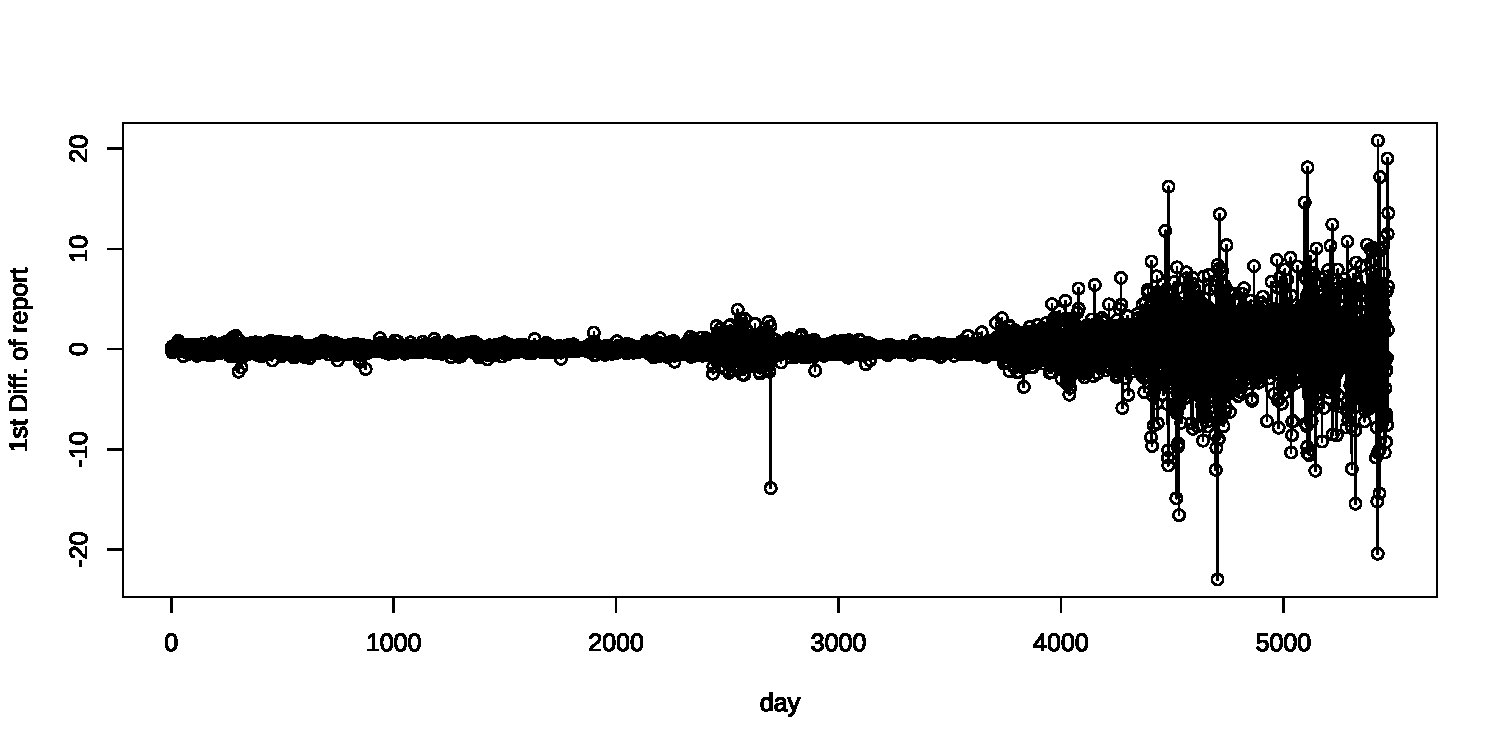
\includegraphics[width=\textwidth]{pic/1dif.pdf} % 插入宽度为文本宽度一半的图片
% 	\caption{一阶差分时序图} % 图片标题
% 	\label{} % 图片标签,用于引用
% \end{figure}
% \FloatBarrier

% \subsection{一阶差分自相关图}
% \begin{lstlisting}
%     acf(as.vector(diff(report,1)),lag.max = 36)
% \end{lstlisting}

% \begin{figure}[h] % 开始一个浮动体环境,[h]指定为 here(这里)位置
% 	\centering % 图片居中
% 	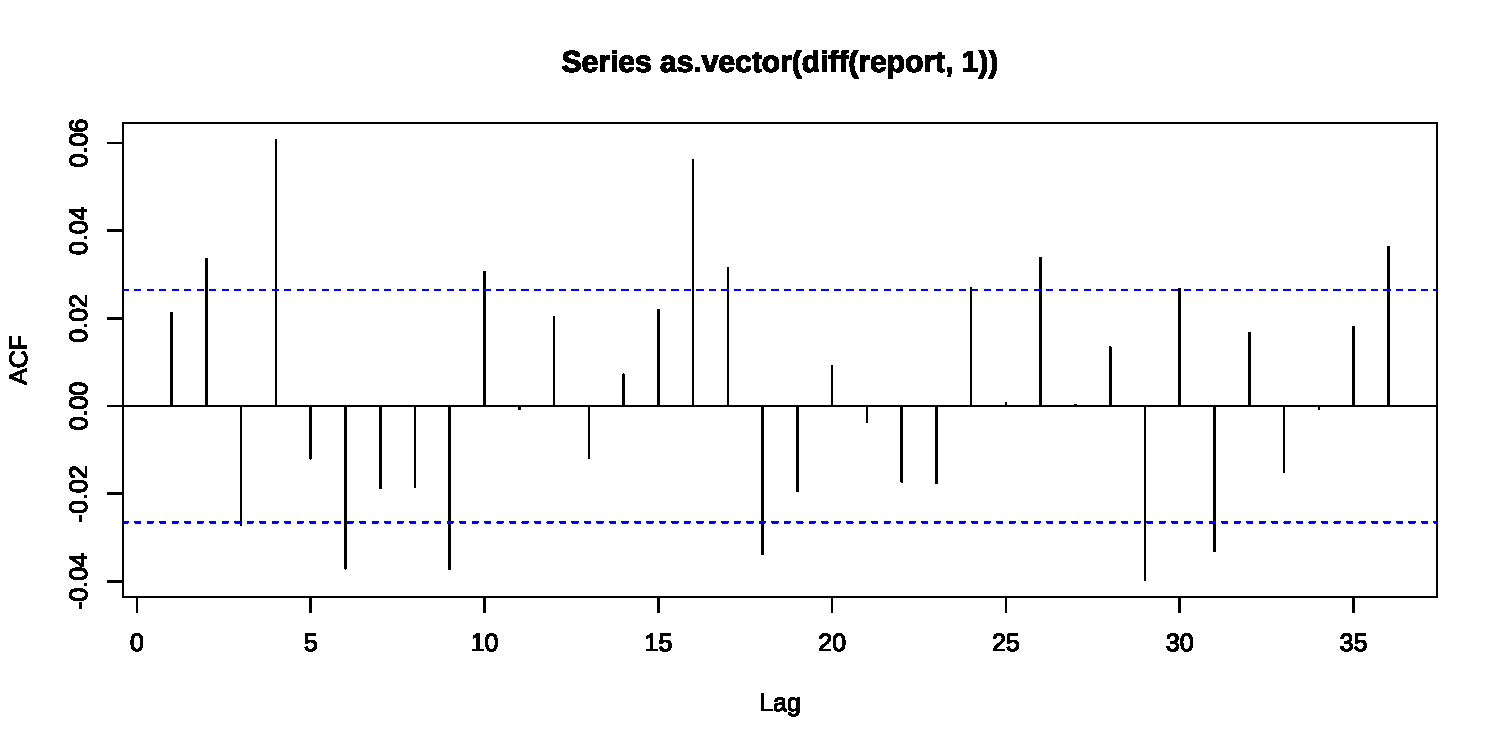
\includegraphics[width=\textwidth]{pic/acf1dif.pdf} % 插入宽度为文本宽度一半的图片
% 	\caption{一阶差分自相关图} % 图片标题
% 	\label{} % 图片标签,用于引用
% \end{figure}
% \FloatBarrier

% \subsection{一阶差分偏自相关图}
% \begin{lstlisting}
%     # 一阶差分偏自相关图
%     pacf(as.vector(diff(report,1)),lag.max = 36)
% \end{lstlisting}

% \begin{figure}[h] % 开始一个浮动体环境,[h]指定为 here(这里)位置
% 	\centering % 图片居中
% 	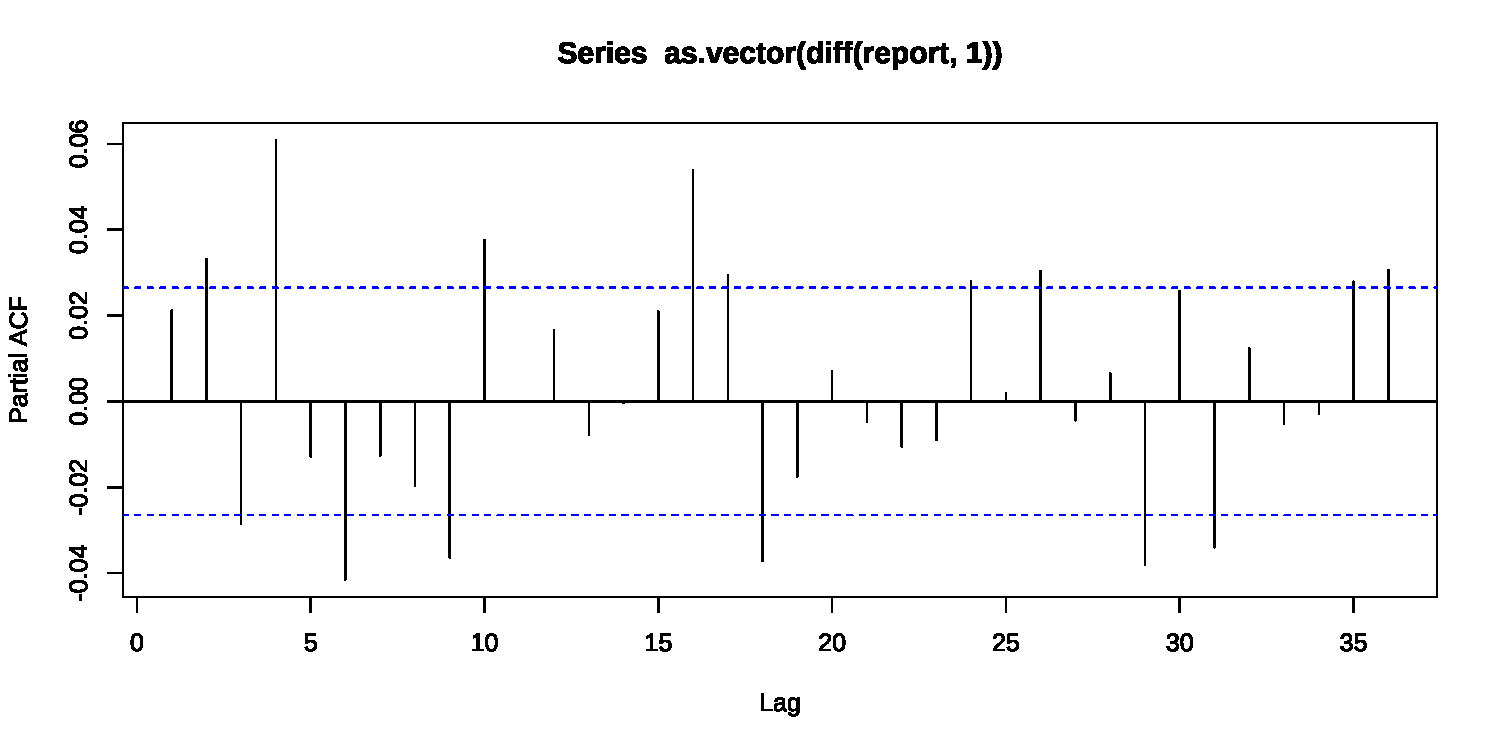
\includegraphics[width=\textwidth]{pic/pacf1dif.pdf} % 插入宽度为文本宽度一半的图片
% 	\caption{一阶差分偏自相关图} % 图片标题
% 	\label{} % 图片标签,用于引用
% \end{figure}
% \FloatBarrier
% 从时序图可得出数据不存在明显的周期性。自相关图中系数没有快速的减为 0,故判断该序列为非平稳序列。

% \subsection{一阶差分 ADF 平稳性检验}
% 为使以上结论更具说服力故调用 adf.test()函数,观察序列是否平稳。

% \begin{lstlisting}
%     # 一阶差分 adf 平稳性检验
%     adf.test(diff(report,1))
%     ## Warning in adf.test(diff(report, 1)): p-value smaller than printed p-value
%     ##
%     ## Augmented Dickey-Fuller Test
%     ##
%     ## data: diff(report, 1)
%     ## Dickey-Fuller = -16.532, Lag order = 17, p-value = 0.01
%     ## alternative hypothesis: stationary
% \end{lstlisting}

% p-value 小于 0.05,拒绝原假设,即该时间序列为平稳序列。

% \subsection{利用EACF确定ARIMA模型阶数}

% Extended Autocorrelation Function (EACF) 成为了我们识别合适ARIMA模型阶数的有力工具。EACF方法,以其独特的矩阵形式,为我们提供了直观的视觉辅助,帮助判断模型中自回归(AR)与移动平均(MA)部分的最优阶数。基于这一理念,我们对苹果公司股票价格序列的一阶差分进行了EACF分析,以期找到最能贴合数据特性的模型配置。

% \begin{lstlisting}
%     eacf(as.vector(diff(report,1)),ar.max=6,ma.max=5)

% \end{lstlisting}
% \begin{table}[h]
%     \centering
%     \begin{tabular}{|c|c|c|c|c|c|c|}
%     \hline
%     AR/MA & 0 & 1 & 2 & 3 & 4 & 5 \\
%     \hline
%     0 & o & x & x & x & o & x \\
%     \hline
%     1 & x & x & \cellcolor{yellow}\textcolor{red}{o} & x & o & o \\
%     \hline
%     2 & x & x & \cellcolor{yellow}\textcolor{red}{o} & x & x & x \\
%     \hline
%     3 & x & x & x & x & x & o \\
%     \hline
%     4 & x & x & x & x & x & o \\
%     \hline
%     5 & x & x & x & x & x & o \\
%     \hline
%     6 & x & x & x & x & x & x \\
%     \hline
%     \end{tabular}
%     \caption{AR/MA关系表}
%     \label{tab:ar-ma-relations}
% \end{table}

% 细观EACF图,我们注意到ARIMA模型的潜在阶数组合。具体而言,表中“o”标记表示模型在该阶数上的可能性较大,而“x”则暗示了相应阶数的不适用性。通过分析,我们发现当AR阶数为1或2,MA阶数为2时,模型表现出了较好的拟合度,这意味着序列可能遵循\(\text{ARIMA}(1,0,2)\)或\(\text{ARIMA}(2,0,2)\)的模型结构。

% 此外,由于我们已知序列在差分后表现为平稳,此处的差分阶数应调整为1,以反映序列的实际特性,因此最终模型应考虑为\(\text{ARIMA}(1,1,2)\)或\(\text{ARIMA}(2,1,2)\)。

% \section{建立模型}

% 为了进一步确定模型是\(\text{ARIMA}(1,1,2)\)和\(\text{ARIMA}(2,1,2)\)中的哪一个,我们比较了一系列统计指标加以确定。

% \subsection{模型拟合}

% 利用 ARIMA 函数进行 ARIMA(1,0,2)拟合
% \begin{lstlisting}
%     ar1_model <- auto.arima(diff(report), max.order = 2, seasonal = FALSE, stationary = TRUE, ic = "aic")
%     summary(ar1_model)
%     ## Series: diff(report) 
%     ## ARIMA(1,0,2) with non-zero mean 
%     ## 
%     ## Coefficients:
%     ##           ar1     ma1     ma2    mean
%     ##       -0.7827  0.8069  0.0562  0.0738
%     ## s.e.   0.1405  0.1400  0.0157  0.0294
%     ## 
%     ## sigma^2 = 4.347:  log likelihood = -11780.49
%     ## AIC=23570.98   AICc=23570.99   BIC=23604.02
%     ## 
%     ## Training set error measures:
%     ##                       ME     RMSE       MAE  MPE MAPE      MASE          ACF1
%     ## Training set 0.001952685 2.084067 0.9756905 -Inf  Inf 0.7126346 -0.0004015358
% \end{lstlisting}

% % 输出给出了模型的系数和标准误差。具体来说,自回归项的系数为0.0214,截距(intercept)的系数为0.0757。它们的标准误差(s.e.)分别为0.0136和0.0288,较小的误差说明了模型拟合得很好。模型的方差估计为4.359,对数似然为-11790.47。这些指标可以用来评估模型的拟合程度,越小的方差和更高的对数似然通常表示模型拟合得更好。AIC可以用于比较不同模型之间的拟合优度,这里输出提供了AIC(赤池信息准则)的值,为23584.94。

% \begin{lstlisting}
%     m010_report<- arima(diff(report), order=c(1, 0, 2), method='ML')
%     print(m010_report)
%     ## 
%     ## Call:
%     ## arima(x = diff(report), order = c(1, 0, 2), method = "ML")
%     ## 
%     ## Coefficients:
%     ##           ar1     ma1     ma2  intercept
%     ##       -0.7840  0.8082  0.0562     0.0753
%     ## s.e.   0.1397  0.1392  0.0157     0.0294
%     ## 
%     ## sigma^2 estimated as 4.343:  log likelihood = -11780.49,  aic = 23568.98
% \end{lstlisting}

% \begin{table}[H]
%     \centering
%     \begin{tabular}{lcccc} % l 表示左对齐的列,c 表示居中对齐的列
%     \toprule % 顶部的加粗横线
%     & ar1 & ma1 & ma2 & intercept \\
%     \midrule % 分割线,比\toprule和\bottomrule细
%     参数估计 & -0.7840 & 0.8082 & 0.0562 & 0.0753 \\
%     参数标准误差 & 0.1397 & 0.1392 & 0.0157 & 0.0294 \\
%     \bottomrule % 底部的加粗横线
%     \end{tabular}
%     \caption{ARIMA(1,0,2)模型参数估计及其标准误差}
%     \label{tab:arima-param-estimates-transposed}
% \end{table}

% \begin{table}[H]
%     \centering
%     \begin{tabular}{lccc} % l 表示左对齐的列,c 表示居中对齐的列
%     \toprule % 顶部的加粗横线
%     & $\sigma^2$ 估计 & 对数似然 & AIC \\
%     \midrule % 分割线,比\toprule和\bottomrule细
%     值 & 4.343 & -11780.49 & 23568.98 \\
%     \bottomrule % 底部的加粗横线
%     \end{tabular}
%     \caption{ARIMA(1,0,2)统计量值}
%     \label{tab:statistics-values-transposed}
% \end{table}

% \begin{table}[H]
%     \centering
%     \begin{tabular}{lccccc} % l 表示左对齐的列,c 表示居中对齐的列
%     \toprule % 顶部的加粗横线
%     & ar1 & ar2 & ma1 & ma2 & intercept \\
%     \midrule % 分割线,比\toprule和\bottomrule细
%     参数估计 & -0.4852 & 0.4485 & 0.5068 & -0.4038 & 0.0754 \\
%     参数标准误差 & 0.2191 & 0.2178 & 0.2244 & 0.2217 & 0.0300 \\
%     \bottomrule % 底部的加粗横线
%     \end{tabular}
%     \caption{ARIMA(2,0,2)模型参数估计及其标准误差}
%     \label{tab:arima-parameters-transposed}
% \end{table}

% \begin{table}[H]
%     \centering
%     \begin{tabular}{lccc} % l 表示左对齐的列,c 表示居中对齐的列
%     \toprule % 顶部的加粗横线
%     & $\sigma^2$ 估计 & 对数似然 & AIC \\
%     \midrule % 分割线,比\toprule和\bottomrule细
%     值 & 4.343 & -11780.16 & 23570.32 \\
%     \bottomrule % 底部的加粗横线
%     \end{tabular}
%     \caption{ARIMA(2,0,2)统计量值}
%     \label{tab:statistics-transposed}
% \end{table}

% 下面针对这两个拟合之后的结果进行比较。

% 首先看参数估计的标准误差,较小的标准误差通常意味着更精确的参数估计。因此由图中可以看出ARIMA(1,0,2)的参数标准误差普遍小于ARIMA(2,0,2)的误差。同时这两个模型的方差估计值,即残差项的方差均为4.343这一数据说明,观测值与模型预测值之间的差异都比较小。我们再来看两者对数似然值的比较,对数似然值描述了给定模型下观测数据出现的概率。因此对于对数似然值而言,越大越好。从表格中我们看到ARIMA(1,0,2)模型的对数似然值为-11780.49,而ARIMA(2,0,2)模型的对数似然值为-11780.16。因此,在这一指标上,ARIMA(2,0,2)模型略优于ARIMA(1,0,2)模型。最后从AIC值分析,ARIMA(1,0,2)模型的AIC值为23568.98,而ARIMA(2,0,2)模型的AIC值为23570.32。由于AIC值越小越好,因此ARIMA(1,0,2)模型在AIC值上的表现也好于ARIMA(2,0,2)模型。


% \subsection{参数的显著性检验}
% 参数的显著性检验:用估计出的系数除以其的标准差(s.e.)得到的商与 T 统计量 5\%临界值 1.96 比较,商的绝对值大于 1.96,则拒绝原假设,认为系数显著的不为 0,否则认为系数不显著。系数不显著的可以去掉。

% \[ t_{统计量(ar1)} = \frac{-0.7827}{0.1405} \approx -5.57,\text{显著} \]

% \[ t_{统计量(ma1)} = \frac{0.8069}{0.1400} \approx 5.76,\text{显著} \]

% \[ t_{统计量(ma2)} = \frac{0.0562}{0.0157} \approx 3.58,\text{显著} \]

% \subsection{残差的正态性检验}
% 画出残差的 QQ 图即可判断,QQ 图中残差基本完全落在 45°线上即为符合正态性假设。否则模型可能出现错误。

% \begin{lstlisting}
%     qqnorm(m121.report$residuals,main='Q-Q 图')
%     qqline(m121.report$residuals)
% \end{lstlisting}

% \begin{figure}[H]
%     \begin{minipage}[t]{0.5\linewidth}
%     \centering
%     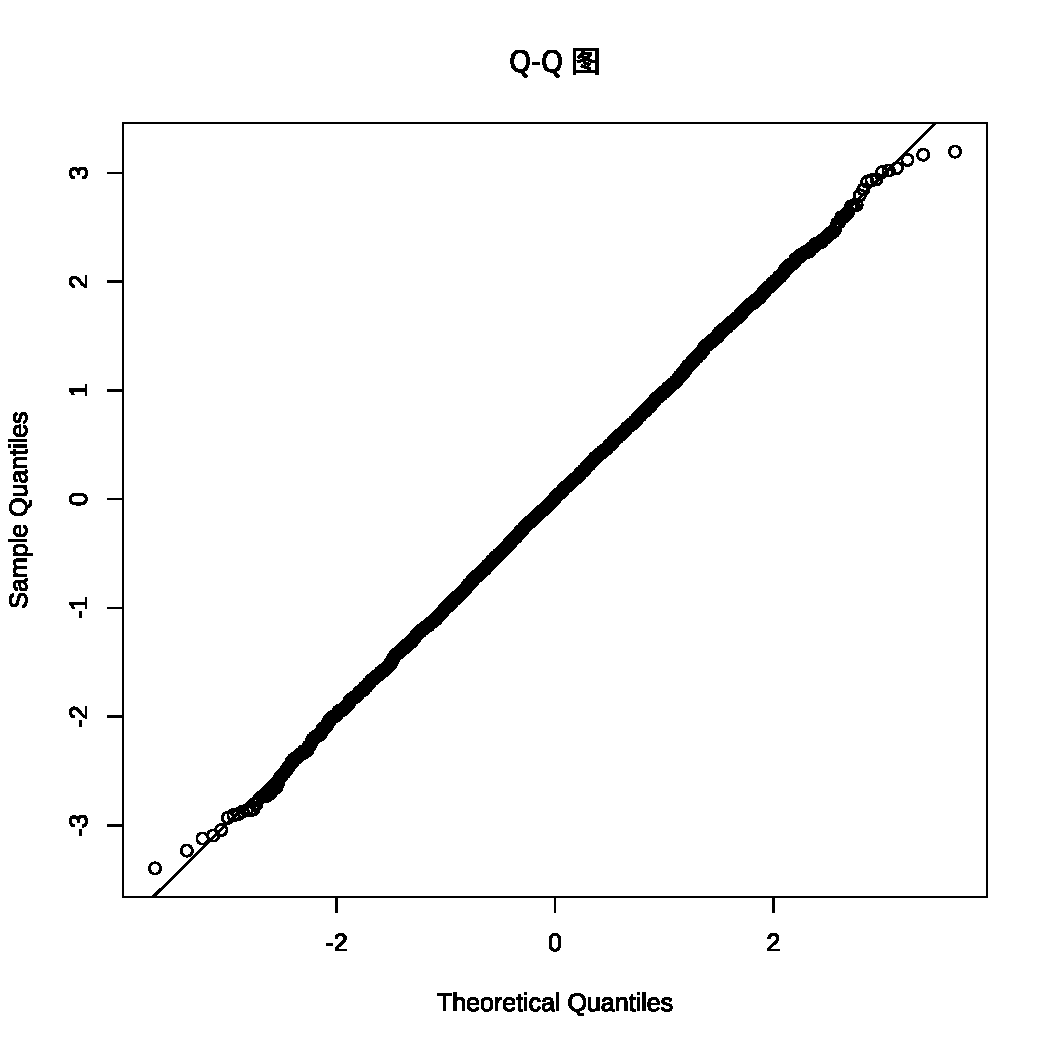
\includegraphics[width=2.2in]{pic/qq_fake.pdf}
%     \caption{ARIMA(1,0,2) Q-Q图}
%     \label{fig:side:a}
%     \end{minipage}%
%     \begin{minipage}[t]{0.5\linewidth}
%     \centering
%     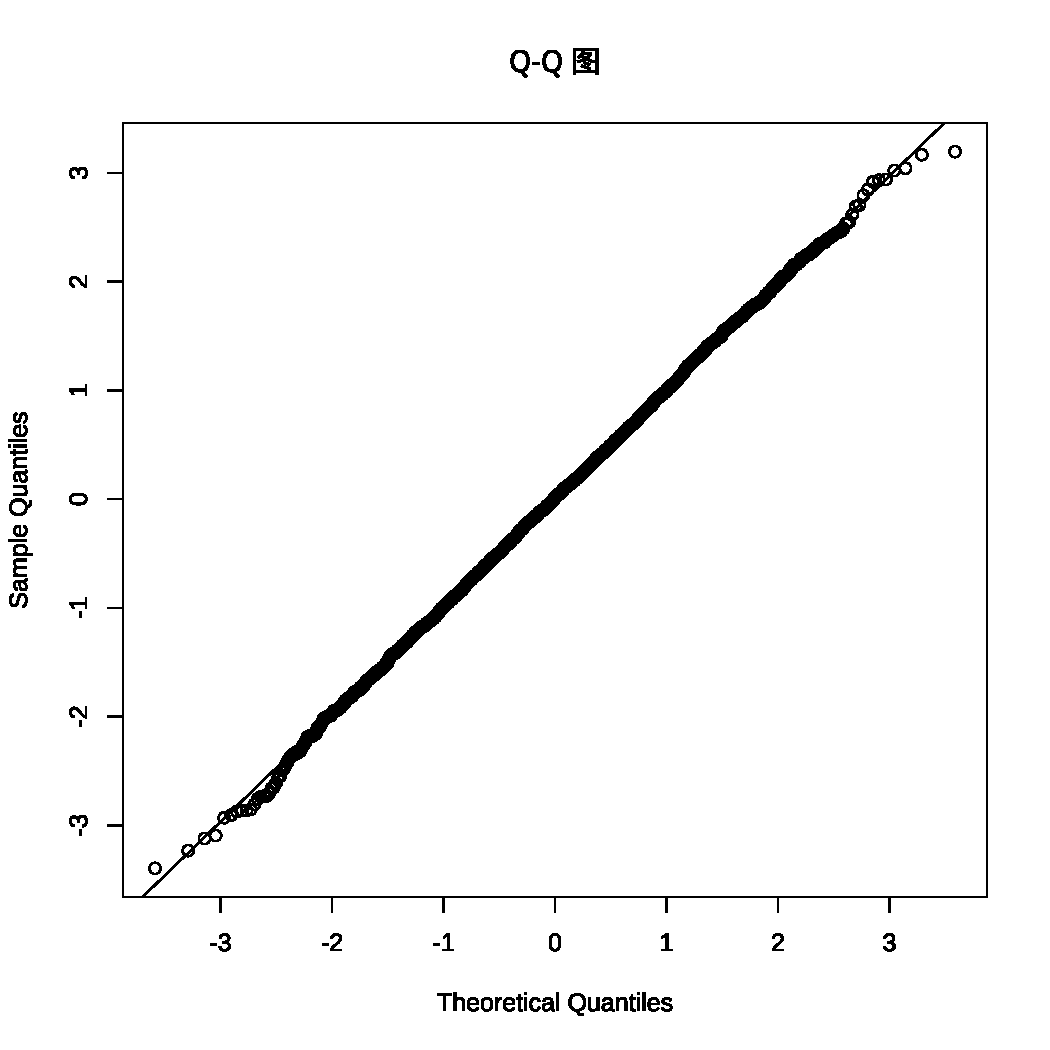
\includegraphics[width=2.2in]{pic/qq_fake1.pdf}
%     \caption{ARIMA(2,0,2) Q-Q图}
%     \label{fig:side:b}
%     \end{minipage}
% \end{figure}

% \subsection{残差的自相关函数图和偏自相关函数图}
% \begin{lstlisting}
%     # 计算 ARIMA(1, 0, 2) 模型的残差
%     residuals <- resid(m010_report)
    
%     # 绘制残差的自相关函数图
%     acf(residuals, lag.max = 36)
% \end{lstlisting}

% \begin{figure}[H] % 开始一个浮动体环境,[h]指定为 here(这里)位置
% 	\centering % 图片居中
% 	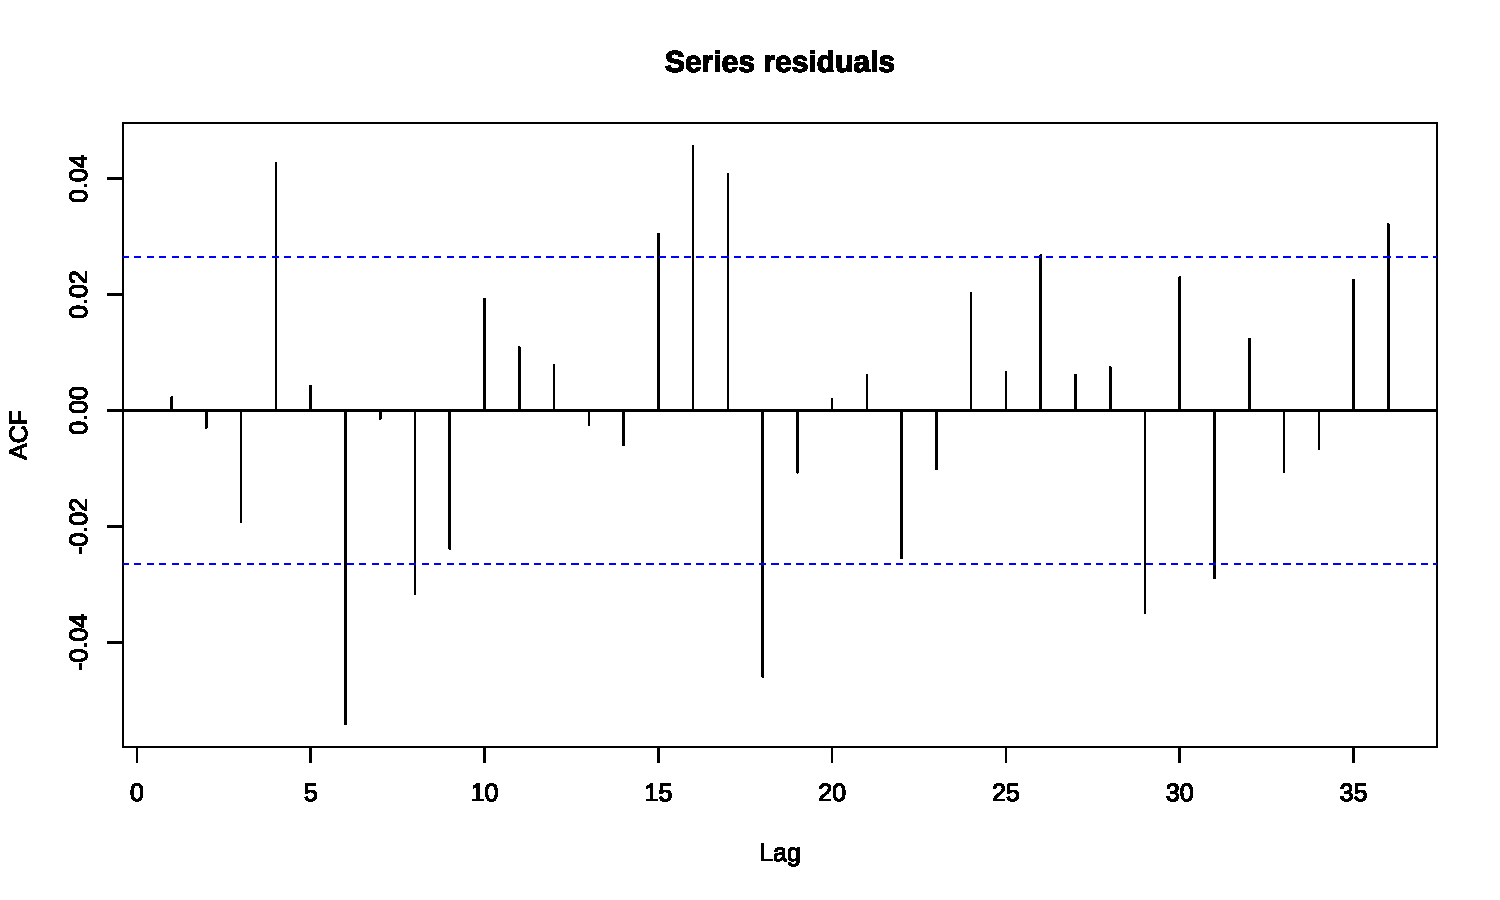
\includegraphics[width=0.75\textwidth]{pic/resacf.pdf} % 插入宽度为文本宽度一半的图片
% 	\caption{残差的自相关函数图} % 图片标题
% \end{figure}

% \begin{lstlisting}
%     # 一阶差分偏自相关图
%     pacf(residuals, lag.max = 36)
% \end{lstlisting}

% \begin{figure}[H] % 开始一个浮动体环境,[h]指定为 here(这里)位置
% 	\centering % 图片居中
% 	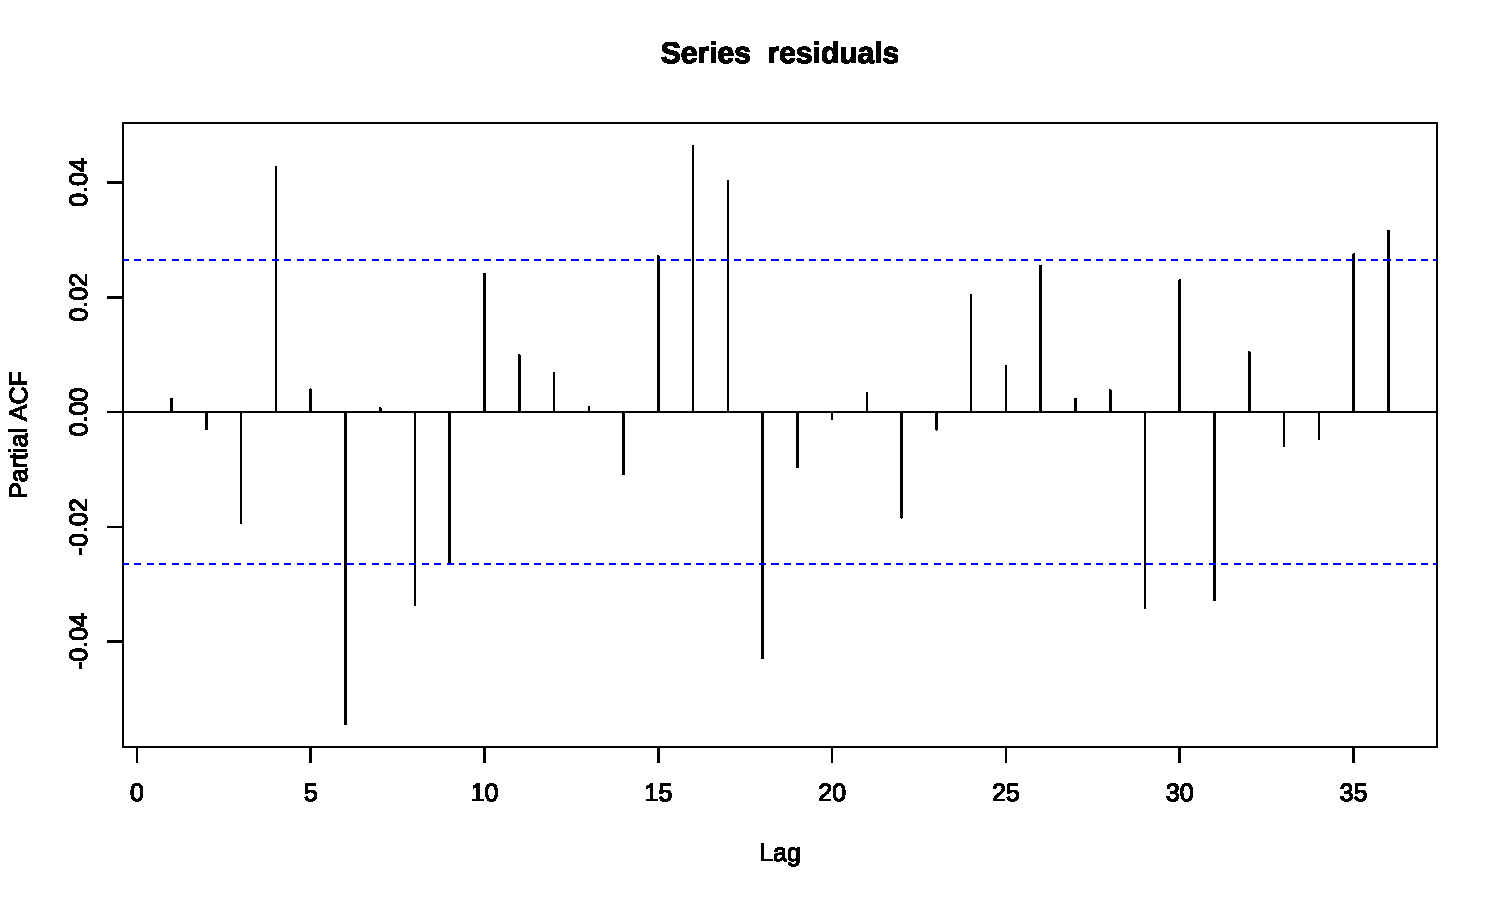
\includegraphics[width=0.75\textwidth]{pic/respacf.pdf} % 插入宽度为文本宽度一半的图片
% 	\caption{残差的偏自相关函数图} % 图片标题
% \end{figure}

% 做出两个模型的ACF和PACF图发现,两个模型的ACF和PACF均呈拖尾。


% \subsection{残差的白噪声检验}
% 白噪声检验作为模型残差分析的核心组成部分,其重要性不言而喻。白噪声序列,定义为一系列独立同分布的随机变量,其均值为零,方差保持恒定,且任意两个不同时间点上的变量之间不存在相关性。在时间序列分析的语境下,当模型残差被证明遵循白噪声分布时,这标志着序列中所有可预测的、系统性的信息已被模型充分提取,剩余的仅是随机扰动,即那些无法通过现有模型结构捕捉的不确定性成分。

% 利用 Ljung-Box 对一阶差分序列的残差进行白噪声检验。如果 \(p<0.05\),拒绝原假设,说明原始序列存在相关性;如果 \(p \geq 0.05\),接受原假设,说明原始序列独立,纯随机,残差是白噪声。
% \begin{lstlisting}
%     Box.test(m010_report$residuals,type="Ljung-Box")
%     ##  Box-Ljung test
%     ## data:  m010_report$residuals
%     ## X-squared = 0.00087885, df = 1, p-value = 0.9763
% \end{lstlisting}

% \begin{table}[H]
%     \centering
%     \begin{tabular}{ll} % l 表示左对齐的列
%     \toprule % 顶部的加粗横线
%     模型 & p-value \\
%     \midrule % 分割线,比\toprule和\bottomrule细
%     ARIMA(1,0,2) & 0.9763 \\
%     ARIMA(2,0,2) & 0.8676 \\
%     \bottomrule % 底部的加粗横线
%     \end{tabular}
%     \caption{ARIMA模型的p-value}
%     \label{tab:model-pvalues}
% \end{table}

% 两个模型的 p-value 分别为 0.9763 和 0.8676,大于 0.05,因此序列的残差为白噪声,原始序列独立,纯随机。

% 综合以上分析,我们可以得出结论:ARIMA(1,0,2)相对于ARIMA(2,0,2)在对数似然函数值和AIC准则下表现更好,说明它能够更好地拟合训练数据,并且前者在模型复杂度更低的情况下取得了更好的表现。因此,在这两个模型中,第一个模型更具有解释力和预测能力。故选择第一个模型进行最后的预测。



% % p-value 为 0.9583,大于 0.05,因此该序列的残差为白噪声,原始序列独立,纯随机。

% \section{模型预测}

% 利用最终确定的ARIMA模型,我们对未来一年内的苹果公司股票价格进行了预测,绘制了预测图,为市场参与者提供了有价值的参考信息。此研究不仅增强了我们对苹果股票动态的洞察力,也展现了时间序列分析在预测金融市场的实用性与潜力。

% 本次研究之旅,我们秉持着严谨的学术态度与系统化的分析方法,深入探索了苹果公司股票价格波动的本质,揭示了其背后隐含的复杂动态与规律性。借助于时间序列分析这一强大工具,我们不仅捕捉到了苹果公司股票价格随时间演进的细微脉络,还构建了一套精确的预测模型,旨在为投资者提供前瞻性的市场洞见。尤为重要的是,我们通过对残差序列的细致检验,确保了模型的稳健性与可靠性,为后续的市场预测创造了更加全面的视角。

% \begin{lstlisting}
%     fit =stats::arima(report,order=c(1,1,2))
%     plot(forecast(fit,365))
% \end{lstlisting}

% \begin{figure}[H] % 开始一个浮动体环境,[h]指定为 here(这里)位置
% 	\centering % 图片居中
% 	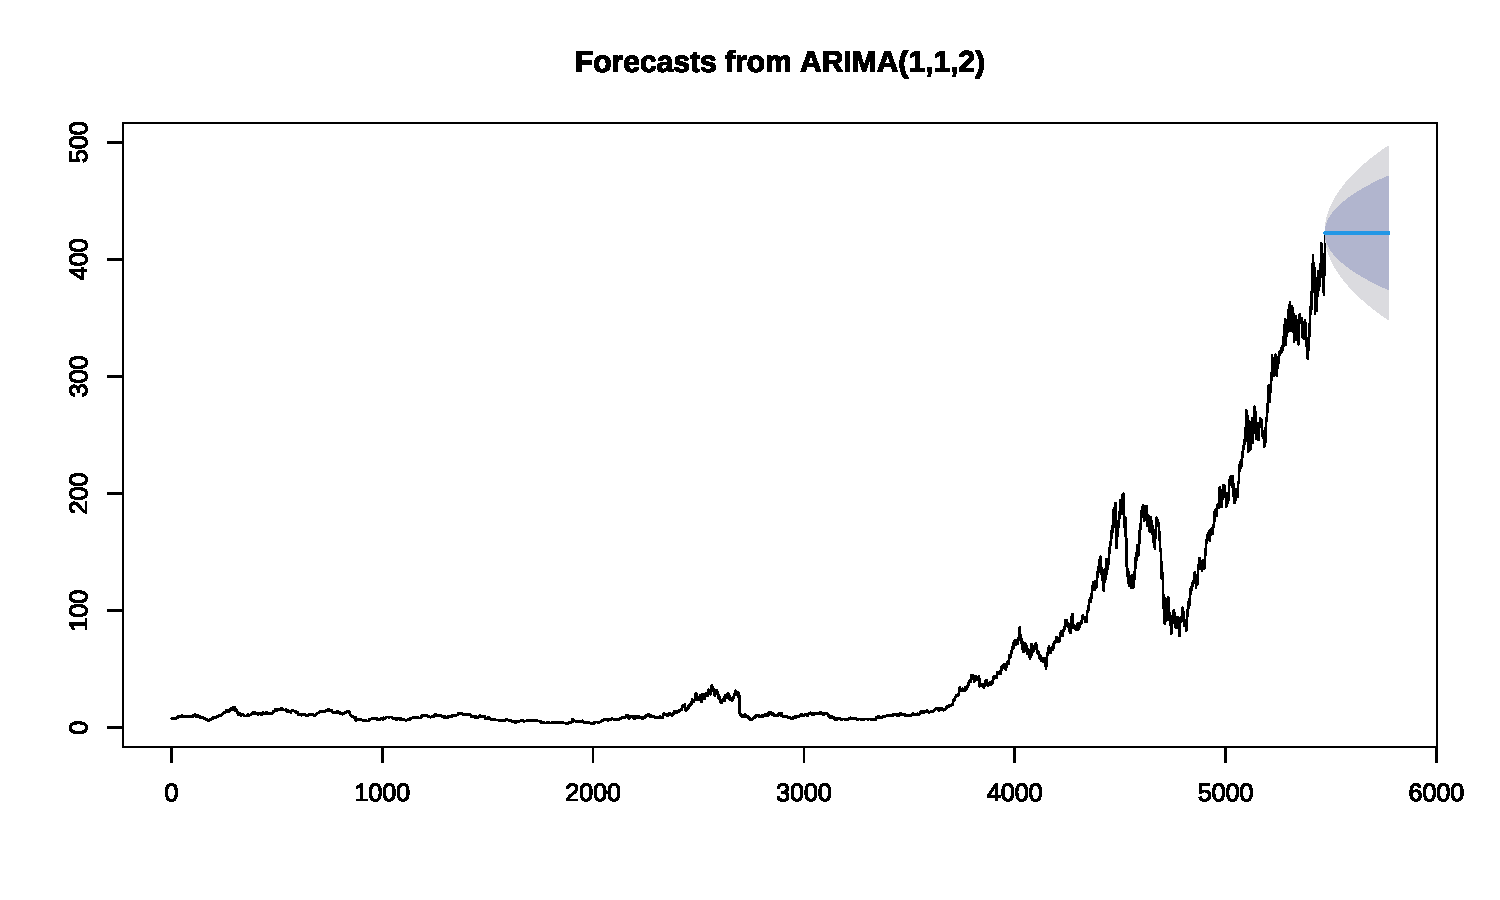
\includegraphics[width=\textwidth]{pic/forecast.pdf} % 插入宽度为文本宽度一半的图片
% 	\caption{模型预测图} % 图片标题
% 	\label{} % 图片标签,用于引用
% \end{figure}
% \FloatBarrier


\end{document}